\documentclass{beamer}
\usepackage[T2A]{fontenc}       %поддержка кириллицы
\usepackage[utf8]{inputenc}
\usepackage{graphicx}
\usetheme{Frankfurt}

\title{Стабилизация неустойчивых эволюционных систем}
\author{Петров Александр}
\date{5 марта 2015 г.}

\graphicspath{{images/}}
\setbeamertemplate{frametitle}[default][left]

\newcommand{\norm}[1]{\left\lVert#1\right\rVert}
\newcommand{\isum}[2][j]{\sum \limits_{#1=1}^{\infty}{#2}}
\newcommand{\operator}[1]{\mathcal{R}{#1}}
\newcommand{\supp}{\mathop{\mathrm{supp}}}

\renewcommand{\figurename}{Рис.}


\begin{document}
\setbeamertemplate{caption}[numbered]

\begin{frame}
\titlepage
\end{frame}


\begin{frame}
\frametitle{Введение}
\hspace{5mm} В реальных физических процессах неизбежно возникают непредусмотренные флуктуации и поэтому возникает необходимость разработки методов построения управлений, способных реагировать и подавлять возмущения. Управления такого типа называются \emph{управления с обратной связью}. В данной работе решались следующие задачи:
\begin{itemize}
	\item Проанализирована устойчивость линейной параболической системы;
	\item Рассмотрен метод стабилизации линейной параболической системы с постоянными коэффициентами конечномерным локальным управлением с обратной связью; 
	\item Представлены численные примеры, показывающие эффективность данного метода на уравнении теплопроводности, численные примеры неустойчивых стационарных решений уравнения Бюргерса
\end{itemize}
\end{frame}


\begin{frame}
\frametitle{Устойчивость параболической системы}

\begin{block}{}
\begin{equation}\label{dif_form}
u_t = u_{xx} + \alpha u, \quad 0 < x < 1, \quad t > 0
\end{equation}
\end{block}
с начальным и граничными условиями:
\begin{block}{}
\begin{gather}\label{d_control}
u(0, t) = u(1, t) = 0, \\*
u(x, 0) = u_{0}(x) \in L^2(0, 1). \nonumber
\end{gather}
\end{block}

\begin{tabular}{@{\textbullet~}l@{\ }p{3in}}
  \bfseries $\alpha = \pi^2$ : & Устойчиво по Ляпунову, но не устойчиво ассимптотически \\
  \bfseries $\alpha < \pi^2$ : & Ассимпотитески устойчиво \\
  \bfseries $\alpha > \pi^2$ : & Неустойчивое нулевое решение
\end{tabular}

\end{frame}

\begin{frame}
\frametitle{Конструкция оператора управления}
Здесь и далее $H = L_2(0, 1), V = H^1_0(0, 1)$.

\hspace{5mm}Пусть $\omega \subset (0, 1)$, такой что $\bar{\omega} \subset (0, 1)$. Задача стабилизации за счет конечномерных локально распределённых в $\omega$ управлений заключается в построении оператора $\mathcal{R} : H \rightarrow H$ такого, что
\begin{enumerate}
\item $\forall z \in H \quad \supp \operator{z} \subset \omega$,
\item $\dim \operator{(H)} < +\infty$.
\end{enumerate}
И при этом решение задачи 
\begin{block}{}
\begin{gather}
  u_t - u_{xx} - \alpha u = \mathcal{R}u, \\*
  u(0, t) = u(1, t) = 0, \; u(x, 0) = u_{0}(x).
\end{gather}
\end{block}
экспоненциально стремится к нулю при $t \rightarrow + \infty$.
\end{frame}


\begin{frame}
\frametitle{Конструкция оператора управления}

\begin{block}{}
\begin{equation}\label{basis}
	w_j = w_j(x) = \sqrt{2}\sin{(\pi j x)}, \quad x \in (0, 1), \quad j=1, 2,..
\end{equation}
\end{block}

Рассмотрим следующие операторы проектирования : $P_m : H \rightarrow H_m$, $Q_m : H \rightarrow H_m^{\perp}$.

\begin{block}{}
\begin{equation}
	P_m u = \sum \limits_{j=1}^{m} {(u, w_j) w_j}
\end{equation}

\begin{equation}
	Q_m u = (I - P_m)u(x) = \sum \limits_{j=m + 1}^{\infty} {(u, w_j) w_j}
\end{equation}
\end{block}

\end{frame}

\begin{frame}
\frametitle{Конструкция оператора управления}

В качестве оператора стабилизиции будем рассматривать следующий конечномерный оператор

\begin{block}{}
\begin{equation}
	\operator{z} = -r\chi_{\omega}P_mz, \quad r > 0
\end{equation}
\end{block}
Здесь 
\begin{block}{}
	\begin{equation}
    \begin{matrix}
	    \chi_{\omega}(x) & =
	    & \left\{
	    \begin{matrix}
	    0, & \mbox{если } x \notin \omega, \\
	    1, & \mbox{иначе. }
	    \end{matrix} \right.
	    \end{matrix}
    \end{equation}
\end{block}

В работе доказано, что существуют подходящие параметры $m \in \mathbb{N}$, $r = r_m > 0$, при которых $\operator{}$ обеспечивает стабилизацию неустойчивого решения.

\end{frame}


\begin{frame}
\frametitle{Численная реализация алгоритма}
Предложена следующая неявная разностная схема \\
\begin{block}{}
	\begin{equation}\label{scheme}
		\frac{u^{j + 1}_i - u^j_i}{\tau} - \frac{u_{i + 1}^{j + 1} - 2u_{i}^{j + 1} + u_{i - 1}^{j + 1}}{h^2} - \alpha(x) u^{j + 1}_i + r\chi_{\omega}P_m u^j_i = 0
	\end{equation}
\end{block}

Оператор $P_m$ аппроксимирован с помощью формулы Филона\\

\end{frame}


\begin{frame}
\frametitle{Пример устойчивого решения уравнения теплопроводности}

$u(x, 0) = \sin{(\pi x)}$. Фиксируем $\alpha = \pi^2 - 2$, $\omega = [0, 0.2]$. 

\begin{figure}[H]
\centering
\begin{minipage}{.5\textwidth}
  \centering
  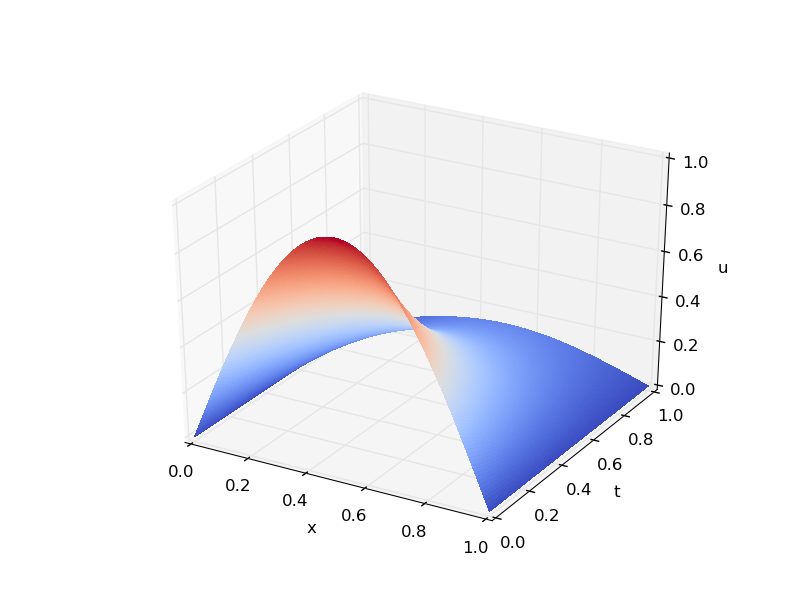
\includegraphics[width=2.4in]{par_ex_pim2}
  \caption{Без управления}
  \label{fig:test1}
\end{minipage}%
\begin{minipage}{.5\textwidth}
  \centering
  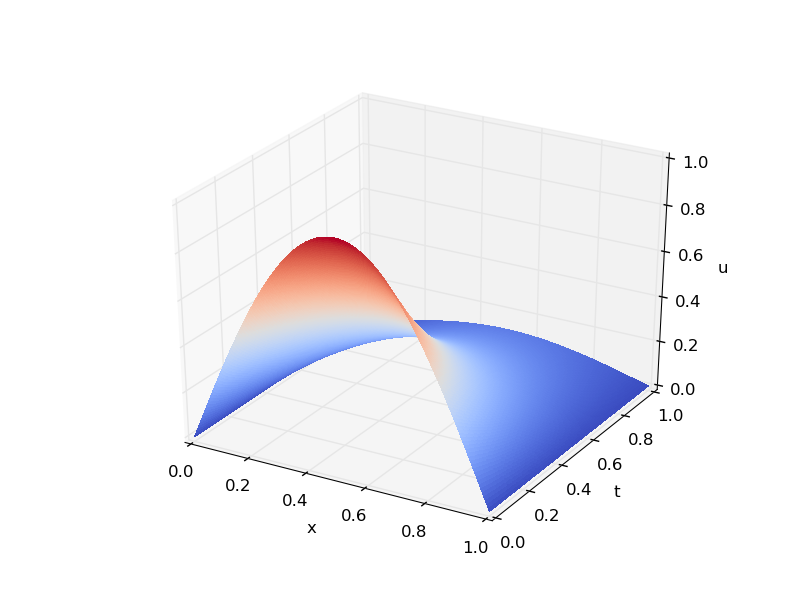
\includegraphics[width=2.4in]{par_re_pim2}
  \caption{Управление $m = 2,\; r = 1$}
  \label{fig:test2}
\end{minipage}
\end{figure}

\end{frame}

\begin{frame}
\frametitle{Пример неустойчивого решения уравнения теплопроводности}

$u(x, 0) = \sin{(\pi x)}$. Фиксируем $\alpha = \pi^2 + 0.1$, $\omega = [0, 0.2]$. 


\begin{figure}[H]
\centering
\begin{minipage}{.5\textwidth}
  \centering
  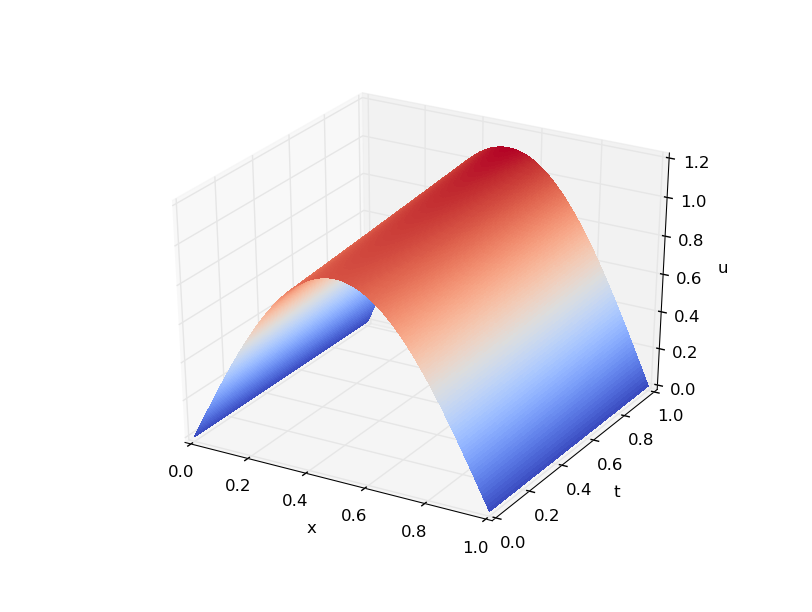
\includegraphics[width=2.4in]{par_ex_pi01}
  \caption{Без управления}
  \label{fig:test1}
\end{minipage}%
\begin{minipage}{.5\textwidth}
  \centering
  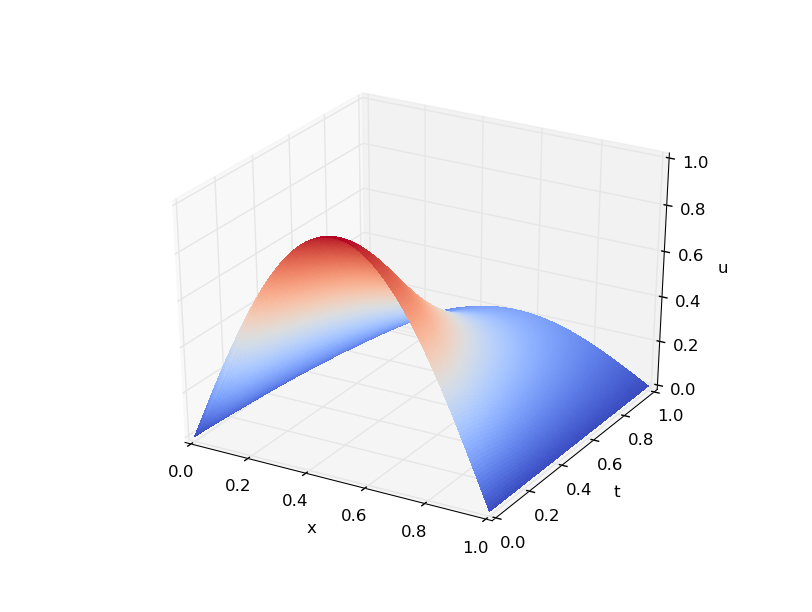
\includegraphics[width=2.4in]{par_re_pi01}
  \caption{Управление $m = 2,\; r = 8$}
  \label{fig:test2}
\end{minipage}
\end{figure}

\end{frame}

\begin{frame}
\frametitle{Пример неустойчивого решения уравнения теплопроводности}

Пусть $u(x, 0) = x(1 - x)$. Фиксируем $\alpha = \pi^2 + 3$, $\omega = [0, 0.4]$. 


\begin{figure}[H]
\centering
\begin{minipage}{.5\textwidth}
  \centering
  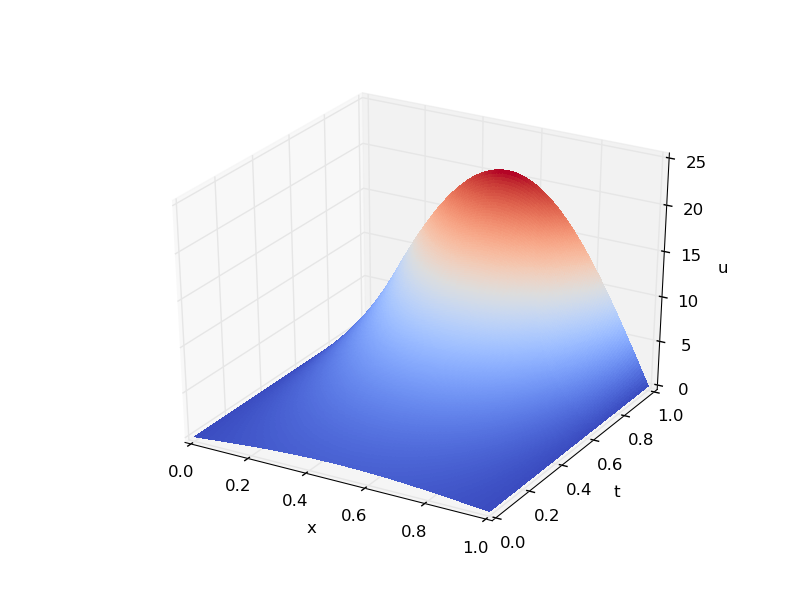
\includegraphics[width=2.4in]{par_ex_pi3}
  \caption{Без управления}
  \label{fig:test1}
\end{minipage}%
\begin{minipage}{.5\textwidth}
  \centering
  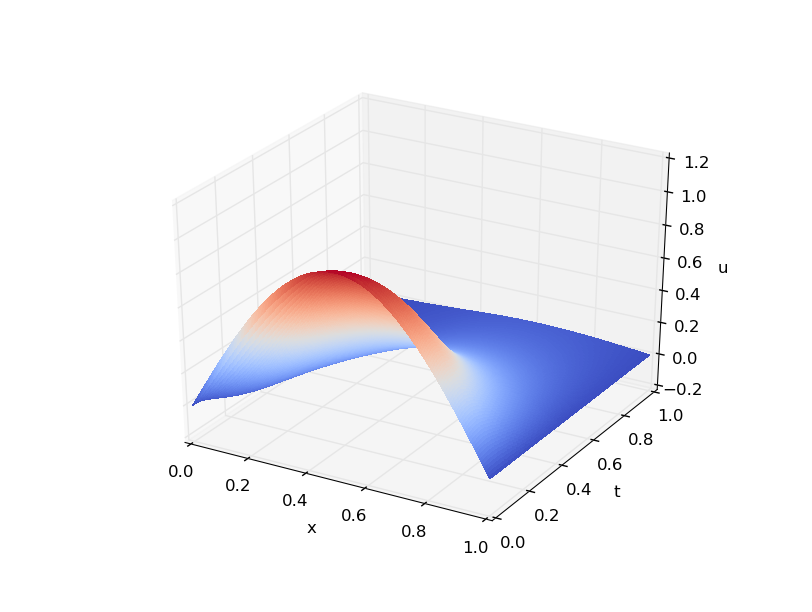
\includegraphics[width=2.4in]{par_re_pi3}
  \caption{$m = 2,\; r = 15$}
  \label{fig:test2}
\end{minipage}
\end{figure}

\end{frame}

\begin{frame}
\frametitle{Стабилизация неустойчивых стационарных решений уравнения Бюргерса}

Рассмотрим вязкое уравнение Бюргерса:
\begin{block}{}
\begin{equation}\label{burger}
  u_t = u_{xx} - u_x u, \quad 0 < x < 1, \quad t > 0
\end{equation}
\end{block}
с начальным и граничными условиями:
\begin{block}{}
\begin{gather}\label{cond}
  u(0, t) = w_1(t), \\*
  u(1, t) = w_2(t), \\*
  u(x, 0) = u_{0}(x) \in L^2(0, 1). \nonumber
\end{gather}
\end{block}

Рассмотрим семейство стационарных решений типа shock-like

\begin{block}{}
\begin{equation}\label{shock_like}
  U(x) = -2\sigma\tanh{(\sigma(x - \frac{1}{2}))},
\end{equation}
\end{block}
где параметр $\sigma \ge 0$.

\end{frame}

\begin{frame}
\frametitle{Стабилизация неустойчивых стационарных решений уравнения Бюргерса}
\begin{figure}[H]
  \centering
  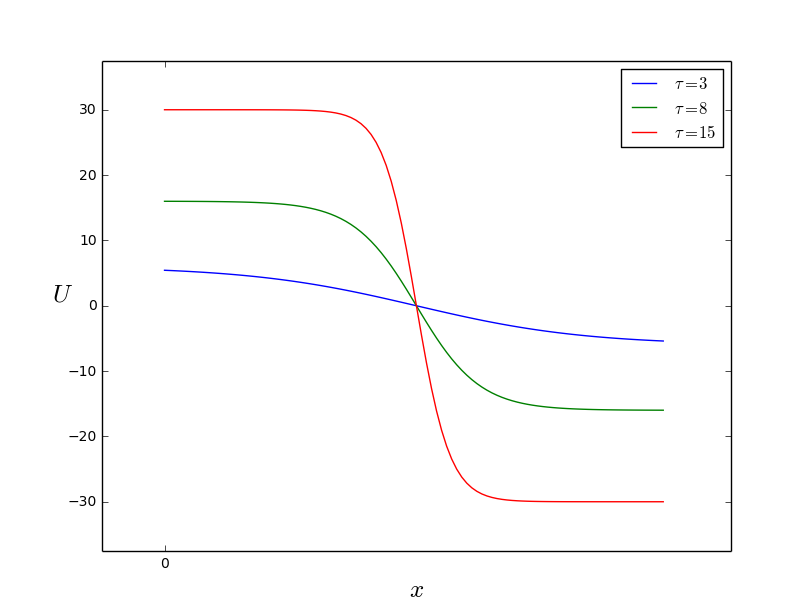
\includegraphics[width=3in]{fig1}
  \caption{$U(x)$ при разных $\sigma$}
\end{figure}
\end{frame}

\begin{frame}
\frametitle{Стабилизация неустойчивых стационарных решений уравнения Бюргерса}
В качестве \eqref{cond} возмем

\begin{block}{}
\begin{gather}\label{cond2}
  w_1(t) = U(0) \\*
  w_2(t) = U(1)
\end{gather}
\end{block}

Введем новое обозначение $\hat{u}(x, t) = u(x, t) - U(x)$. Тогда, система \eqref{burger} перепишется через новую переменную $\hat{u}$

\begin{block}{}
\begin{gather}\label{fluct}
    \hat{u}_t = \hat{u}_{xx} - U(x)\hat{u}_x - U'(x)\hat{u} - \hat{u}_x\hat{u}, \\*
    \hat{u}(0, t) = \hat{u}(1, t) = 0, \\*
    \hat{u}(x, 0) = u_{0}(x) - U(x) \in L^2(0, 1).
\end{gather}
\end{block}

\end{frame}

\begin{frame}
\frametitle{Стабилизация неустойчивых стационарных решений уравнения Бюргерса}

Для изучения устойчивости системы \eqref{fluct}, линеаризуем её

\begin{block}{}
\begin{gather}\label{linearized}
  \theta_t = \theta_{xx} + 2 \sigma (\tanh(\sigma(x - \frac{1}{2}))\theta)_x \\*
  \theta(0, t) = \theta(1, t) = 0,
\end{gather}
\end{block}

где $\theta(x, t)$ линеаризация $\hat{u}$. \eqref{linearized} - уравнение конвенкции-диффузии-реакции. Для простоты изучения устойчивости, мы избавимся от конвекционого члена используя преобразование $\zeta(x, t) = G(x)\theta(x, t)$, где 

\begin{block}{}
\begin{equation}
  G(x) = \frac{\cosh(\sigma(x - \frac{1}{2}))}{\cosh(\frac{\sigma}{2})}
\end{equation} 
\end{block}

\end{frame}

\begin{frame}
\frametitle{Стабилизация неустойчивых стационарных решений уравнения Бюргерса}

\begin{block}{}
\begin{gather} \label{transf_linear}
  \zeta_t = \zeta_{xx} + \sigma^2 \left( \frac{2}{\cosh^2(\sigma(x - \frac{1}{2}))} - 1 \right) \zeta \\* 
  \zeta(0) = \zeta(1) = 0 
\end{gather}
\end{block}

Для $\sigma = 0$ система нейтрально устойчива. Для $\sigma > 0$, реакционный член в \eqref{transf_linear} также является неустойчивым в окрестности $x = \frac{1}{2}$ (Рис 2.).

\end{frame}

\begin{frame}
\frametitle{Стабилизация неустойчивых стационарных решений уравнения Бюргерса}

\begin{figure}[H]
  \centering
  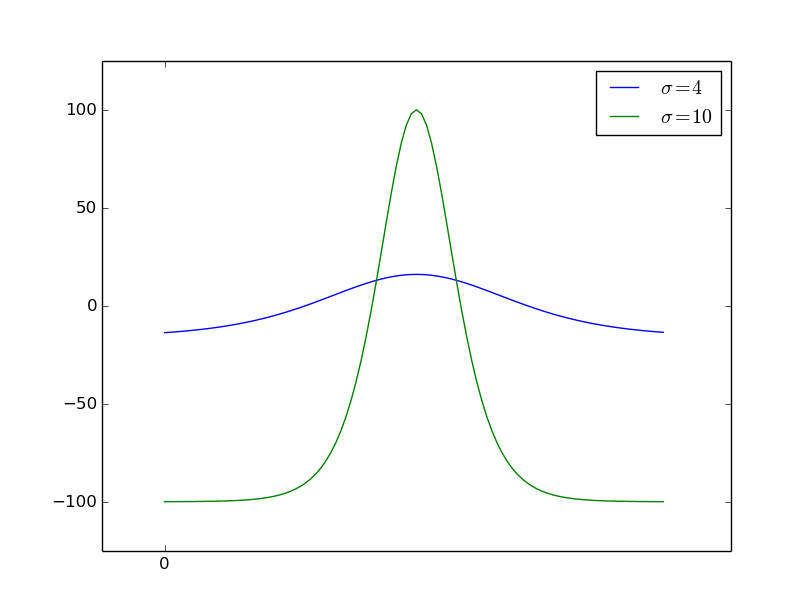
\includegraphics[width=3in]{fig2}
  \caption{$\frac{2}{\cosh^2(\sigma(x - \frac{1}{2}))} - 1$}
\end{figure}

\end{frame}

\begin{frame}
\frametitle{Примеры неустойчивых стационарных решений уравнения Бюргерса}

Пусть $\theta_0(x) = \frac{\sin(\pi x)}{G(x)}$. Фиксируем $\omega = [0, 0.2]$, $\sigma = 3$. 


\begin{figure}[H]
\centering
\begin{minipage}{.5\textwidth}
  \centering
  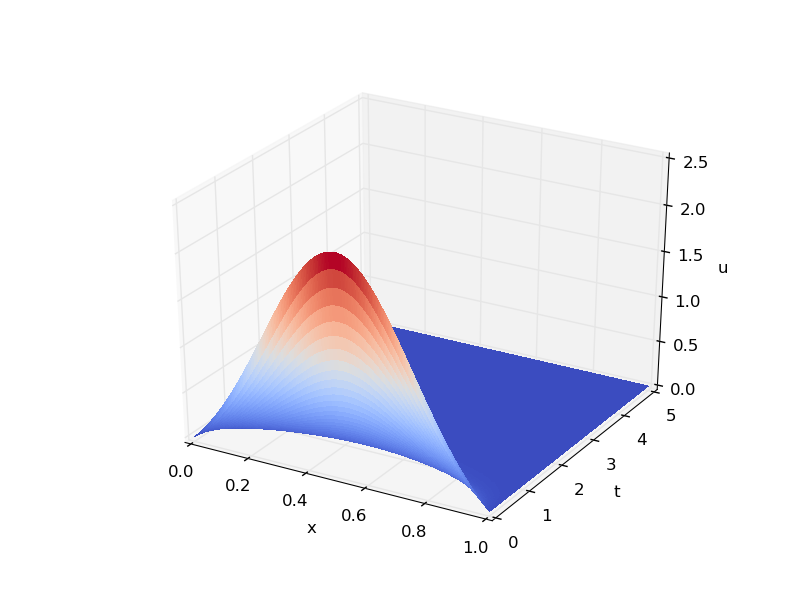
\includegraphics[width=2.4in]{ex_s3}
  \caption{Без управления}
  \label{fig:test1}
\end{minipage}%
\begin{minipage}{.5\textwidth}
  \centering
  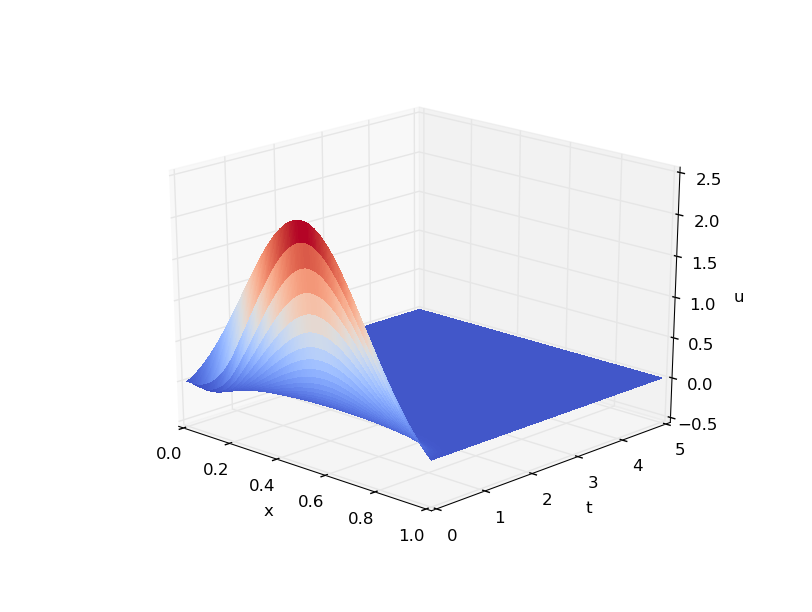
\includegraphics[width=2.4in]{re_s3}
  \caption{$m = 2, \; r = 15$}
  \label{fig:test2}
\end{minipage}
\end{figure}

\end{frame}

\begin{frame}
\frametitle{Примеры неустойчивых стационарных решений уравнения Бюргерса}

$\theta_0(x) = \frac{\sin(\pi x)}{G(x)}$. Фиксируем $\omega = [0, 0.2]$, $\sigma = 15$. 


\begin{figure}[H]
\centering
\begin{minipage}{.5\textwidth}
  \centering
  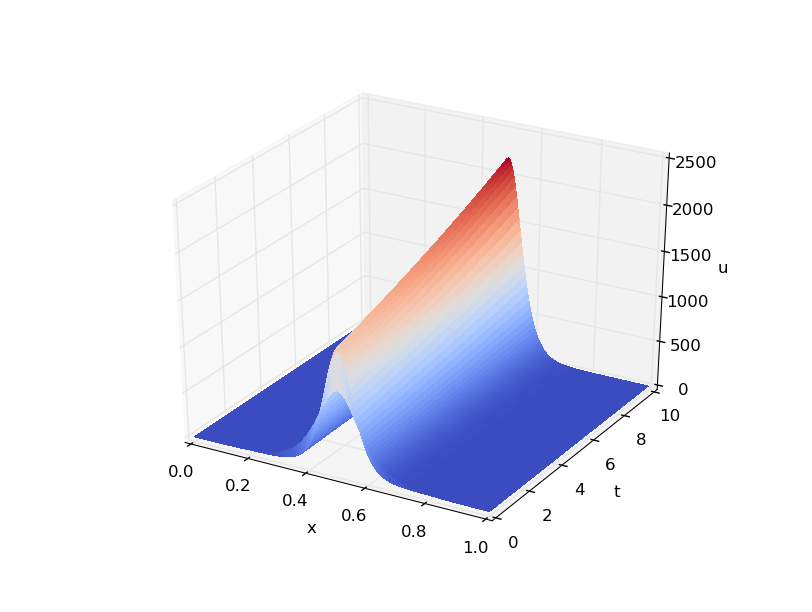
\includegraphics[width=2.4in]{ex_s15}
  \caption{Без управления}
  \label{fig:test1}
\end{minipage}%
\begin{minipage}{.5\textwidth}
  \centering
  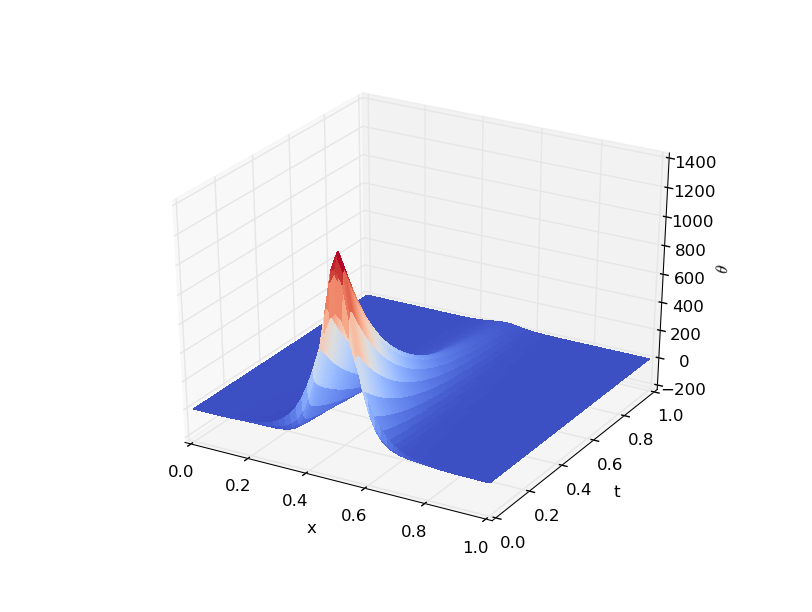
\includegraphics[width=2.4in]{re_s15}
  \caption{Управление с $m = 2, \; r = 15$}
  \label{fig:test2}
\end{minipage}
\end{figure}


\end{frame}

\begin{frame}
\frametitle{Примеры неустойчивых стационарных решений уравнения Бюргерса}

В качестве начального условия возмем быстро осциллирующую функцию $\frac{\sin(10 \pi x)}{G(x)}$. Параметр $\sigma$ возмем равным 15. 



\begin{figure}[H]
\centering
\begin{minipage}{.5\textwidth}
  \centering
  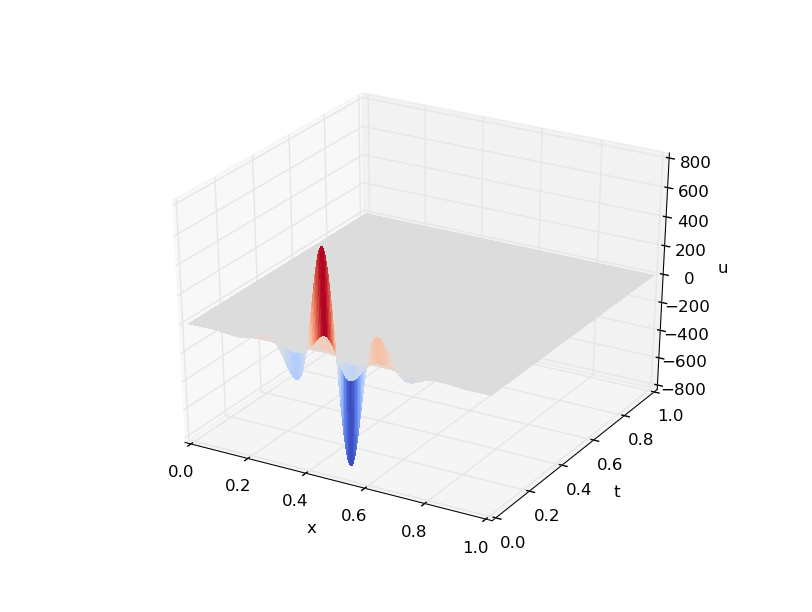
\includegraphics[width=2.4in]{ex_sin10_s15}
  \caption{Без управления}
  \label{fig:test1}
\end{minipage}%
\begin{minipage}{.5\textwidth}
  \centering
  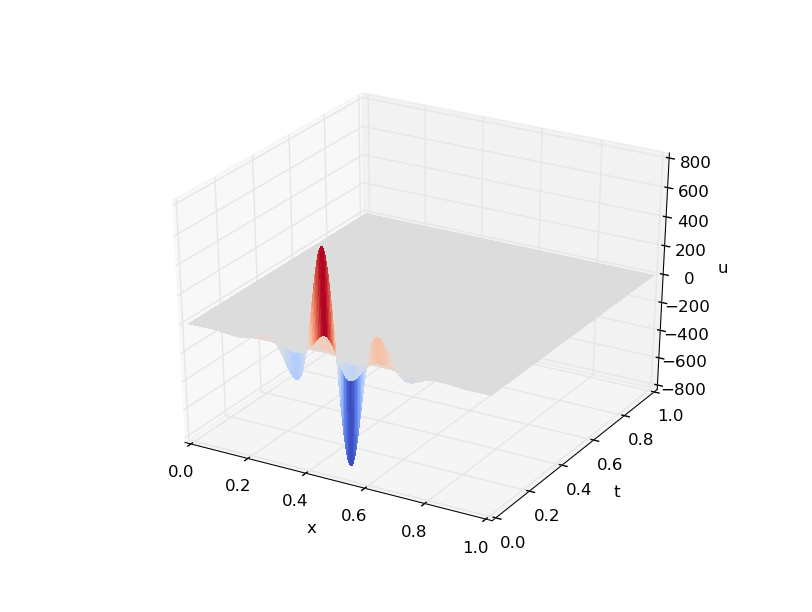
\includegraphics[width=2.4in]{re_sin10_s15}
  \caption{Управление с $m = 2, \; r = 15$}
  \label{fig:test2}
\end{minipage}
\end{figure}


\end{frame}


\begin{frame}
\frametitle{Примеры неустойчивых стационарных решений уравнения Бюргерса}

$\theta_0(x) = \frac{x^2}{G(x)}$. Фиксируем $\omega = [0, 0.2]$, $\sigma = 15$. 


\begin{figure}[H]
\centering
\begin{minipage}{.5\textwidth}
  \centering
  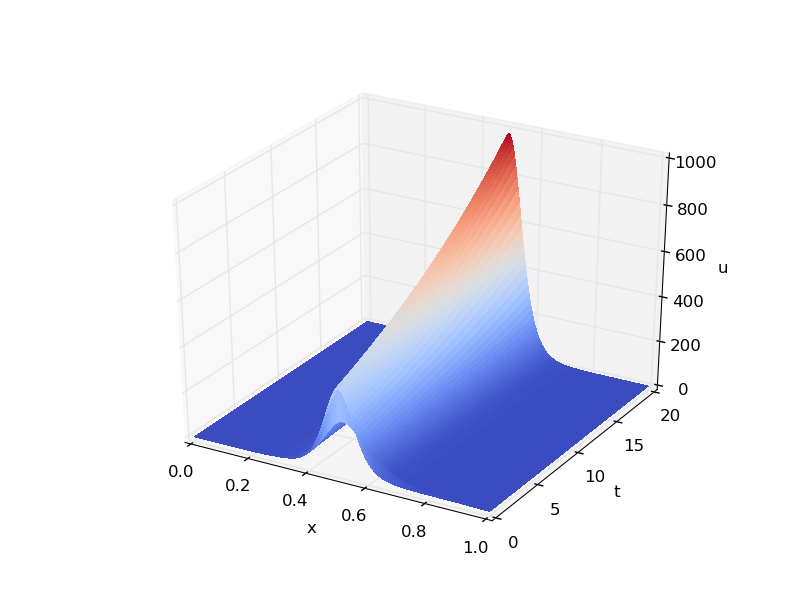
\includegraphics[width=2.4in]{ex_x2_s15}
  \caption{Без управления}
  \label{fig:test1}
\end{minipage}%
\begin{minipage}{.5\textwidth}
  \centering
  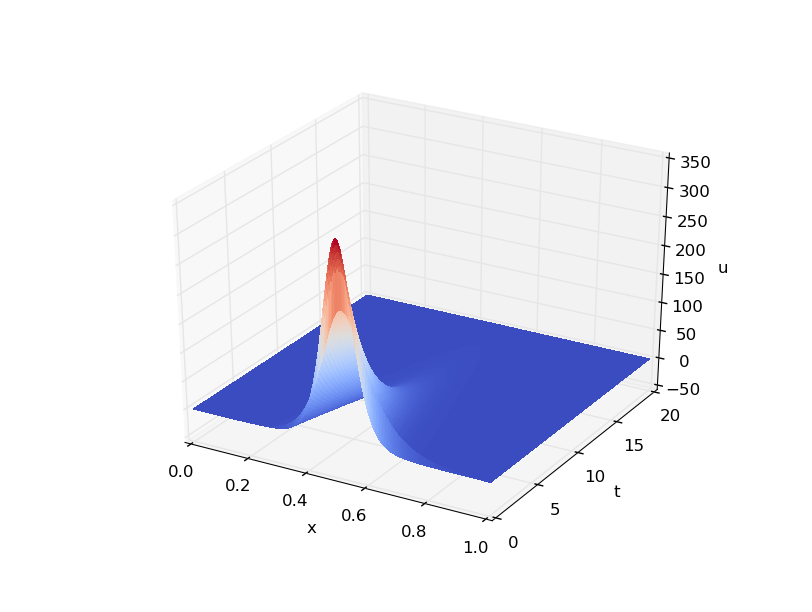
\includegraphics[width=2.4in]{re_x2_s15}
  \caption{$\omega = [0, 0.2], \; r = 15, \; m = 2$}
  \label{fig:test2}
\end{minipage}
\end{figure}



\end{frame}


\begin{frame}
\frametitle{Заключение}

При выполнении цели данной работы были выполнены следующие задачи:
\begin{itemize}
	 \item Изучена литература, связанная с описанием и решением задачи стабилизации параболических систем;
  \item Подробно разобран метод стабилизации локальным конечномерным управлением с обратной связью;
  \item Численная реализация метода стабилизации, в том числе : написание программы для вычисления разностной схемы, метода Филона.
  \item Приведены численные примеры неустойчивых стационарных решений уравнения Бюргерса, применение метода стабилизации.
\end{itemize}

\end{frame}

\begin{frame}
	\begin{center}
	\Huge Спасибо за внимание
	\end{center}
\end{frame}

\end{document}
